\documentclass[letterpaper, 11pt, twoside, captions=tableheading]{scrartcl}
\usepackage[utf8]{inputenc}
\usepackage[default]{sourcesanspro}
\usepackage{sfmath}
\usepackage{amsmath}
\usepackage{amssymb}
\usepackage{amsbsy}
\usepackage{amsthm}
\usepackage{upgreek}
\usepackage{graphicx}
\usepackage{multirow}
\usepackage{geometry}
\geometry{
  left=3.045cm,
  right=2.045cm,
  top=3cm,
  bottom=3cm,
  showframe=true,
}
\usepackage{setspace}
\setstretch{1.5} %line spacing
\usepackage{hyperref}
\hypersetup{
colorlinks,
citecolor=black,
filecolor=black,
linkcolor=black,
urlcolor=black,
linktoc=all,
pdftitle=Physics PhD Preliminary Exam McGill,
pdfauthor=Laurenz Kremeyer,
pdfcreator=Laurenz Kremeyer,
pdfdisplaydoctitle=true,
pdfpagelayout=TwoPageRight
}
\usepackage[style=phys, biblabel=brackets, maxbibnames=2, minbibnames=1, sortlocale=de_DE, doi=false, isbn=false, url=false, doi=false, backend=biber, sorting=none, backref=false]{biblatex}
\DeclareFieldFormat[article]{citetitle}{#1\midsentence}
\DeclareFieldFormat[article]{title}{#1\midsentence}
\DeclareFieldFormat[book]{title}{#1\midsentence}
\DeclareFieldFormat[online]{title}{#1\midsentence}
\addbibresource{refs.bib}
\usepackage[nolist]{acronym}
\usepackage{caption}
\captionsetup[figure]{labelfont={bf},name={Fig.},labelsep=colon}
\captionsetup[table]{labelfont={bf},name={Tab.},labelsep=colon}
\captionsetup[figure]{font={stretch=1.15}}
\captionsetup[table]{font={stretch=1.15}}
\setcapindent{0em}
\setlength\abovecaptionskip{6pt} %spacing between table and its title
\raggedbottom
\emergencystretch=20em

\newcommand{\e}{\mathrm{e}}
\renewcommand{\i}{\mathrm{i}}
\newcommand{\ts}{TiSe\textsubscript{2}}

\begin{document}
\begin{acronym}
\acro{TMD}{transition-metal dichalcogenide}
\acro{BZ}{brillouin zone}
\acro{CDW}{charge-density wave}
\acro{PLD}{periodic lattice distortion}
\acro{DFT}{density functional theory}
\acro{UEDS}{ultrafast electron diffuse scattering}
\acro{UED}{ultrafast electron diffraction}
\acro{LA}{longitudinal acoustic}
\acro{TA}{tansverse acoustic}
\end{acronym}
\section{\ts Literature Review}
\ts\space is a material in the group of \acp{TMD}.
All \ac{TMD} appear in the general form MX\textsubscript{2} with M being a layer of transition-metal atoms such as molybdenum, tungsten or titanium which are sitting between two layers of species X from the group of chalcogens like sulfur or selenium.
This covalently bonded structure is called a \ac{TMD} monolayer.
\Ac{TMD} bulk material is made up of many monolayers stacked monolayers, bonded by van-der-Waals interaction.

The research part of my studies will focus on the \ac{TMD} \textit{1T}-\ts, the \textit{1T}-prefix is referring to the stacking order of the monolayers, that results in octahedrally coordinate
From here on out it will simply be referred to as \ts.
Its crystal structure at room temperature and atmospheric pressure is depicted in figure~\ref{fig:crystal}\,a.
The unit cell contains one Ti atom and two Se atoms and the lattice vectors have lengths of $|\mathbf{a}|=|\mathbf{b}|=3.541$\,\AA\space and $\mathbf{c}=6.001$\,\AA\cite{patel1983}.
The material shows semi-metallic electronic characteristics\cite{bachrach1976}, with a hole pocket from the Se 4s band at the $\Gamma$ point of the \ac{BZ} and an electron pocket at the L point from the Ti 3d band\cite{zunger1978}.

Upon cooling, at 200\,K \cite{disalvo1976} \ts\space undergoes a second order phase transition into a phase with a commensurate $2\times2\times2$ \ac{PLD} accompanied by a \ac{CDW}\cite{rossnagel2011}.
The maximum displacement of the atoms is $u_\mathrm{max}/|\mathbf{a}|=2.4\%$\cite{disalvo1976}.
\ac{CDW} and \ac{PLD} go hand in hand, since a periodic modulation of the electron density will shift the equilibrium positions of the ions.
Vice versa, periodically displaced ions will alter the electron density to more adequately screen their potential.
Currently two mechanisms are discussed to drive the \ac{CDW}/\ac{PLD}: 
Firstly, the band Jahn-Teller effect describing the splitting of two degenerate energy bands due broken symmetry introduced by electron-phonon coupling and electron-lattice interaction\cite{rossnagel2002}.
Secondly, the formation of a excitonic insulator ground state due to cooperative interaction between the charge carriers\cite{kogar2017}.

Theoretical work shows that a \ac{CDW} phase transition driven by the band Jahn-Teller mechanism will be stable in materials with large electron-phonon coupling constants and large electronic susceptibilities\cite{friend1979}.
An alteration of the electron and phonon dispersion in form of a band gap opening at the Fermi surface and a Kohn anomaly are predicted.
A Kohn anomaly will manifest itself as a strong phonon renormalization towards $\omega=0$\cite{kohn1959} (in this case at the M and L points in the \ac{BZ}).
This was previously observed with the very instrument that will be the key part of the proposed research\cite{otto2021}.

\begin{figure}[!t]
	\begin{minipage}{0.5\columnwidth}
		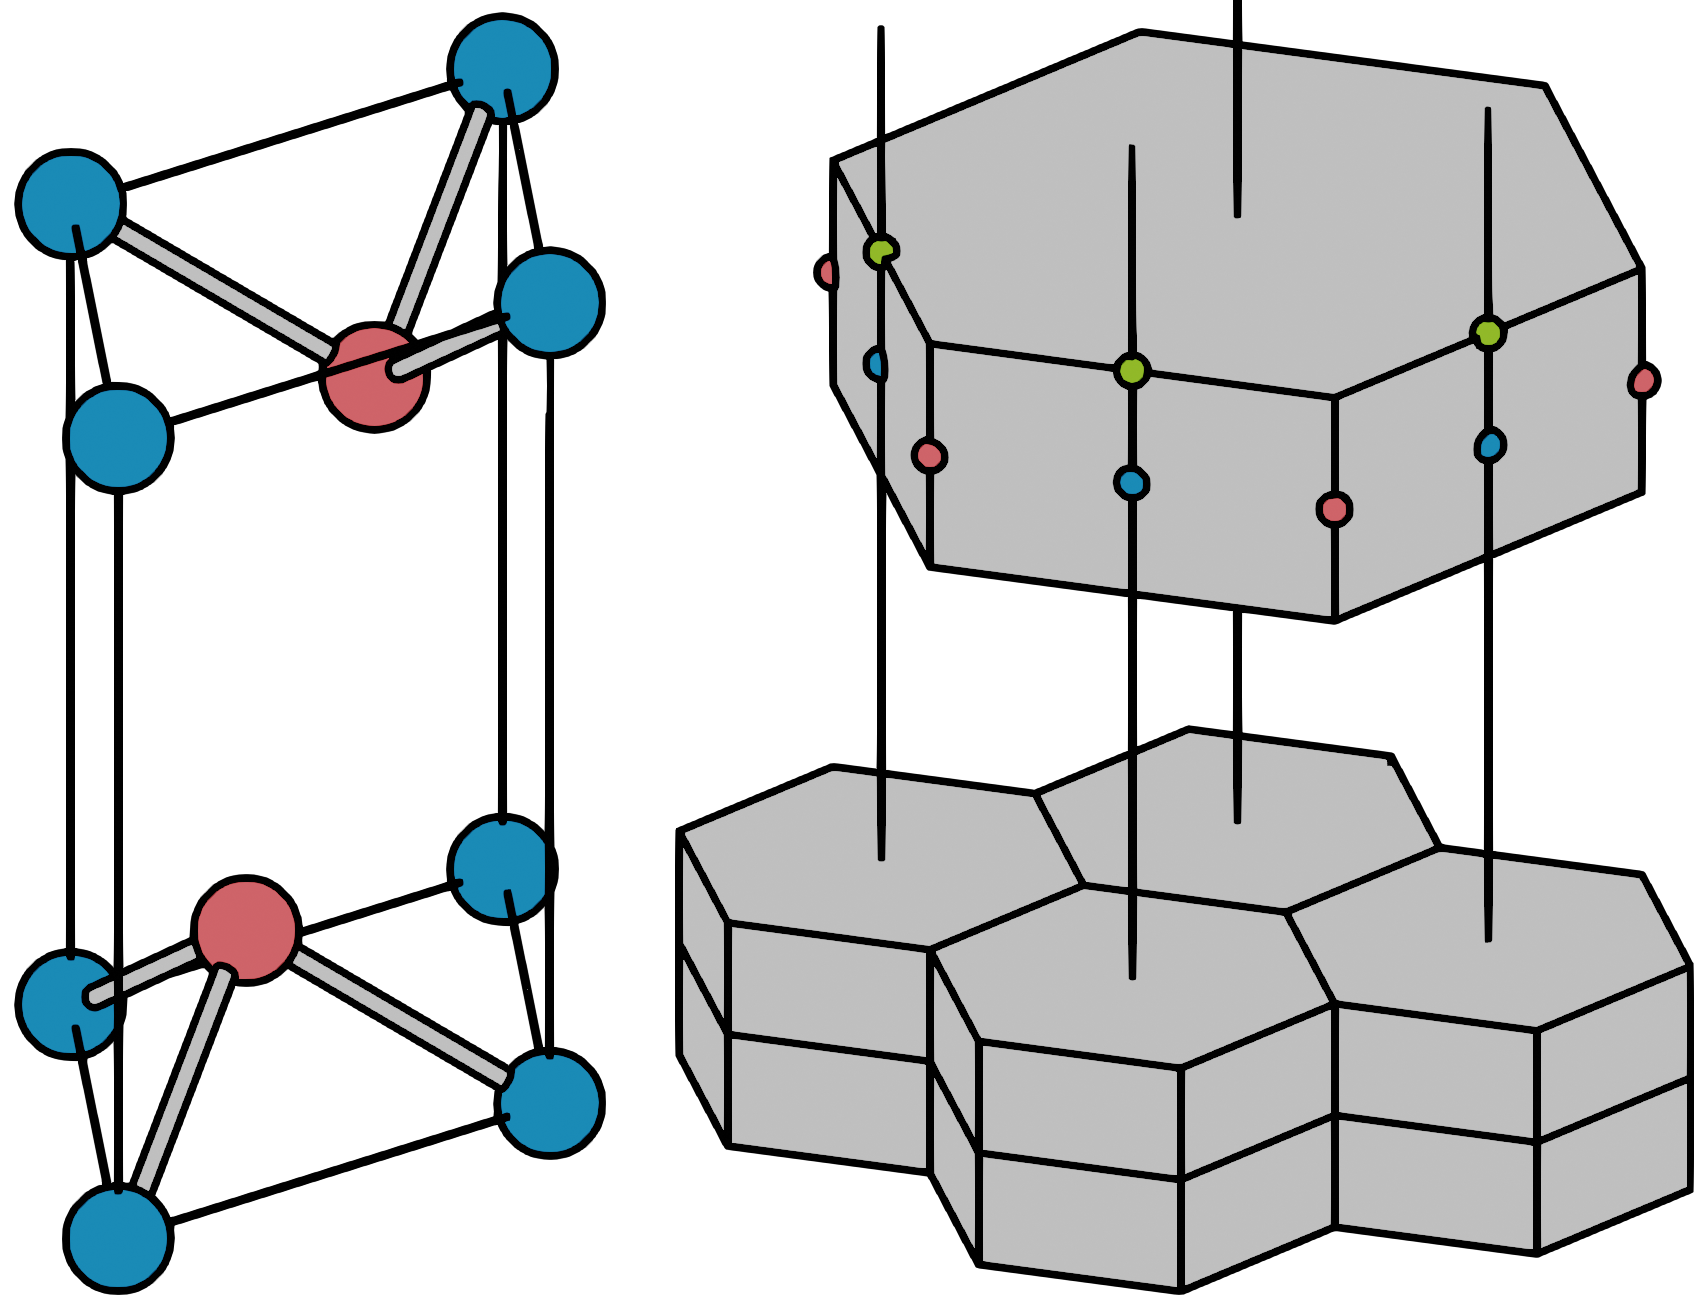
\includegraphics[width=\columnwidth]{figs/tise2_crystal.png}
	\end{minipage}
	\hspace{0.04\columnwidth}
	\begin{minipage}{0.45\columnwidth}
		\caption{\textbf{a)}\,Hexagonal unit cell of \ts, comprised of one Ti atom and two Se atoms. Ti atoms are shown in blue, Se atoms in red. \textbf{b)}\,\ac{BZ} of the high temperature phase (top) and low temperature phase (bottom) of \ts. Blue/red/green spheres mark the positions of M/K/L points in the \ac{BZ}.}
		\label{fig:crystal}
	\end{minipage}
\end{figure}

A phonon with vanishing frequency is often referred to as \emph{frozen} and corresponds to a static \ac{PLD} that does not require energy to form.
Density functional theory (DFT)\acused{DFT} simulations show that the superposition of the three freezing phonon modes at the M points are in good agreement with the experimentally observed \ac{PLD}\cite{kaneko2018}. % if first use is \AC, this thing fails...
The strong electron-phonon coupling in \ts\space results in a large lattice distortion, a large energy gap and a small coherence length of the \ac{CDW} phase\cite{haas1978,hildebrand2016}.

A lower energy ground state created by charge carrier interaction is the so called excitonic insulator state, described by Kohn et al. in \cite{jerome1967, kohn1967}.
Considering a semi-metal with a small indirect band overlap or a semiconductor with a small indirect band gap as shown in figure~\ref{fig:ei}\,a+b).
The small band overlap semi-metal can be seen as an insulator with few charge carriers.
Carriers are poorly screened and holes and electrons are attracting each other through Coulomb interaction, leading to exciton formation.
Exciton formation becomes more energetically favorable for smaller band overlaps starting at a critical overlap of $G_\mathrm{C}$, as shown in figure~\ref{fig:ei}\,c).
Starting from a normal insulator with band gap $G$ and reducing it, the system will at some point reach a state where the size of the band gap is the same as the energy of the lowest-lying exciton, $G-E_\mathrm{B}=0$.
This electronic instability leads to exciton formation, similar to the semi-metallic case.
Thus for $G_\mathrm{C}<G<E_\mathrm{B}$ the excitonic insulator ground state is stable.

Experimentally it is hard to distinguish both mechanisms.
However, analogous to the phonon softening in the band Jahn-Teller state, there will be a soft plasmon in the excitonic insulator state \cite{kohn1967, rossnagel2011}, this has been experimentally confirmed by momentum-resolved electron energy-loss spectroscopy\cite{kogar2017}.
The redistribution of charges inside the material will lead to \ac{CDW} formation, which can produce a \ac{PLD}.

\begin{figure}[!t]
	\begin{minipage}{0.5\columnwidth}
		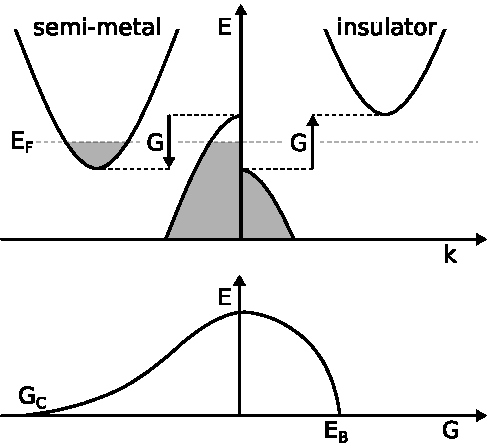
\includegraphics[width=\columnwidth]{figs/excitonic_insulator.pdf}
	\end{minipage}
	\hspace{0.04\columnwidth}
	\begin{minipage}{0.45\columnwidth}
		\caption{Band structure of a indirect semi-metal (\textbf{a}) with a band overlap of $G<0$ and an indirect insulator (\textbf{b}) with an indirect band gap of $G>0$ \textbf{c)} Net energy gain of the new excitonic ground state, between a critical band overlap $G_\mathrm{C}$ and a band gap up to the lowest exciton binding energy $E_\mathrm{B}$}
		\label{fig:ei}
	\end{minipage}
\end{figure}

Although both approaches that have been discussed lead to qualitatively the same \ac{CDW}/\ac{PLD} phase, the underlying mechanisms are quite different.
The latter being driven by electron-electron and electron-hole interaction, whereas the former is mainly driven by strong electron-phonon coupling.

%misc
% describe difference in CDW/PLD from TiSe2 and other materials
% inverse width of kohn annomaly is measure for the coherence length
Studying the dynamics of solid-state systems far from equilibrium with ultrafast experimental techniques has gained attraction over the last decades.
These techniques allow to probe different observables on femtosecond timescales, shedding light on the relaxation pathways towards equilibrium.

\textbf{pump-probe}

A simple concept to reach high time resolutions is the pump-prope technique.
The basic idea is that an excitation event (pump) and a probe event with a known variable time difference occur on the sample under investigation.
The excitation event may be an arriving optical laser pulse and the probe event might be the scattering of an electron or X-ray pulse.
If probe-events are measured while continiously varying the time delay the data can be assembled into a \emph{movie}.
Both, excitation and probe event, are required to be shorter than the time scale of the pheonomenon under investigation.
If the phenomenon under study is reversable and there is enough time between each excitation event, a measurement can be done continiously on one sample.
Current plans do not involve studying irreversible phenomena.

\begin{figure}[!t]
	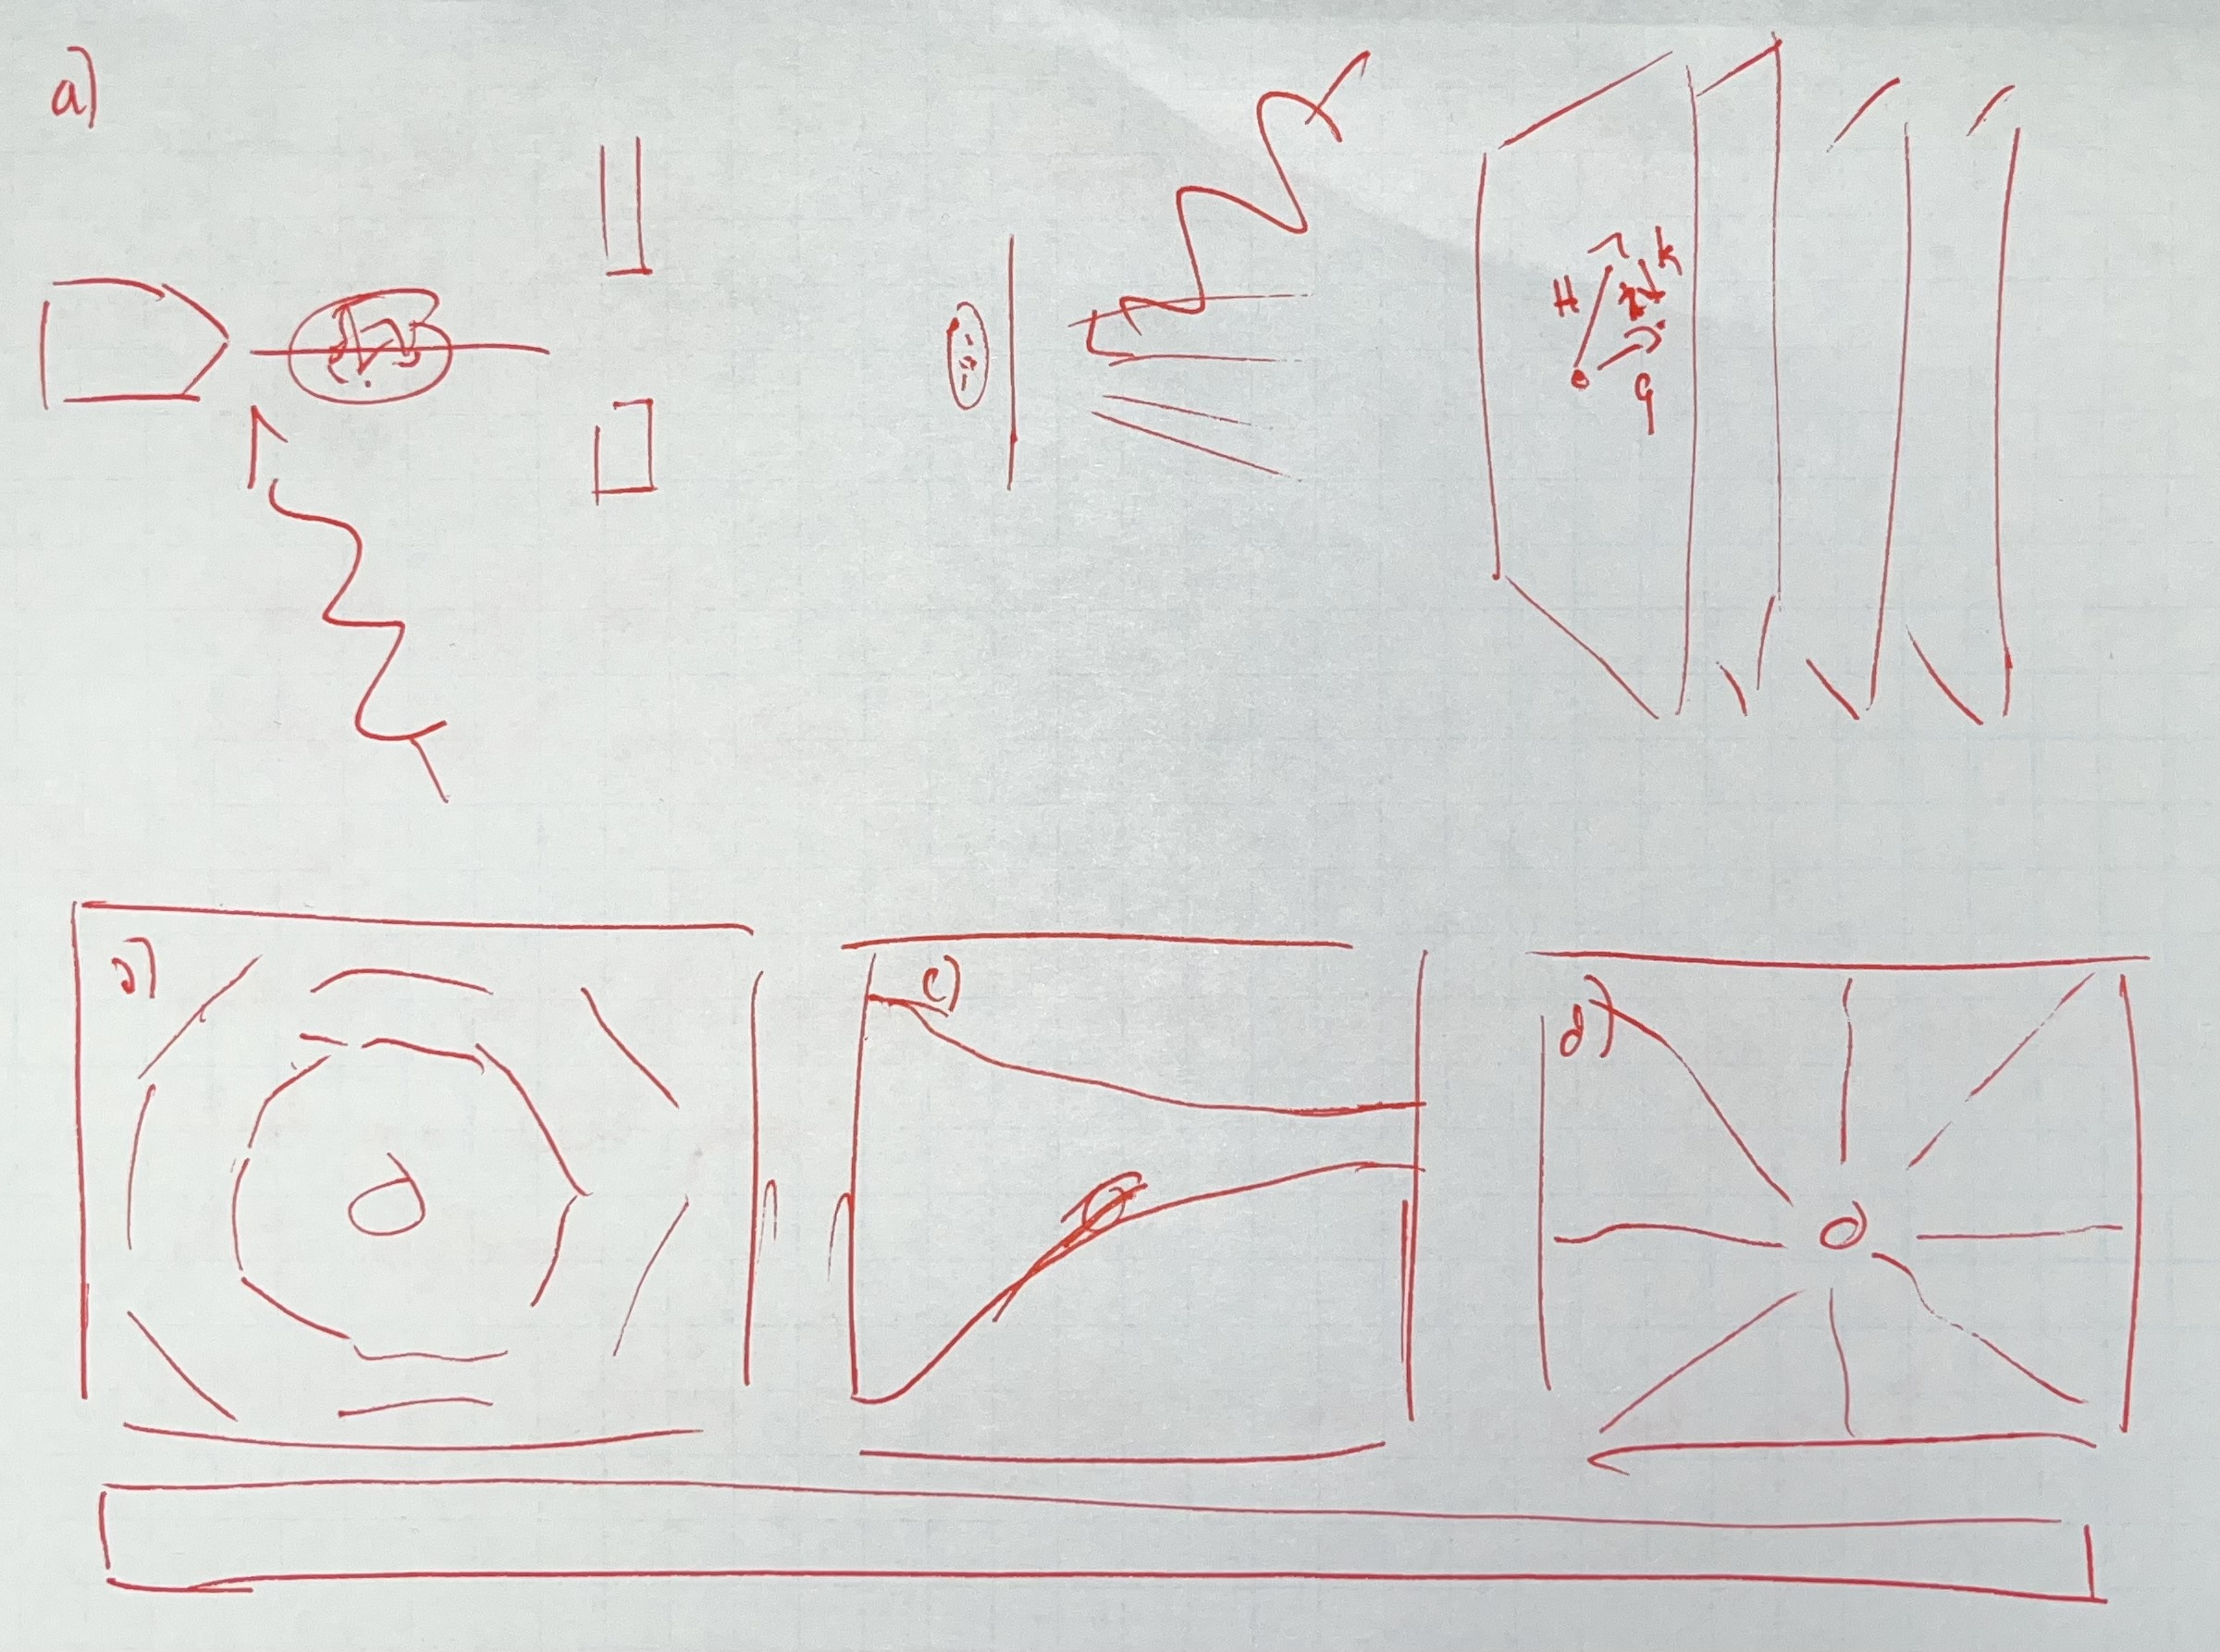
\includegraphics[width=\columnwidth]{figs/method_placeholder.jpg}
	\caption{\textbf{a)}\,Working principal of \acs{UEDS}. The laser pump pulse arrives at the sample, followed by the electron probe pulse with a time delay of $\tau$. The electrons are scattered off of the sample and collected on the detector. For one pixel on the detector the scattering vector $\mathbf{q}$, its reduced wave vector $\mathbf{k}$ and the closest Bragg reflection $\mathbf{H}$ are shown. One-phonon structure factors of the longitudinal (\textbf{b}) and transverse (\textbf{c}) acoustic modes in the high temperature phase of \ts.}
	\label{fig:method}
\end{figure}

\textbf{UED/UEDS}

Building on the idea of the pump-probe scheme one can combine classical electron diffraction experiments and femtosecond laser systems and conduct \ac{UED} and \ac{UEDS} experiments.

The experimental apparatus starts with a commercial Ti:sapphire laser system emitting $\sim$35\,fs laser pulses with a center wavelength of 800\,nm, that are split and guided onto different beam path.
For sample excitation one part of the pulse is attenuated and guided onto the sample.
Part of the pulse entering the probe beam path is frequency doubled. The fundamental and frequency doubled pulses are converted to a pulse with a center wavelength of 266\,nm by frequency summation.
The final pulse is guided onto a photo cathode in vacuum, where the electron bunch that will be scattered from the sample is being created.
The electron bunch is accelerated to 90\,keV by a static electric field and focused onto the sample.
On its way to the sample the electron bunch will broaden considerably due to Coulomb repulsion, effectively limiting the time resolution of the experiments.
To compensate for this effect the electron bunches are re-compressed in a radio-frequency driven cavity between the electron gun and the sample.
A schematic representation is shown in shown in figure~\ref{fig:method}\,a:
Laser pump and electron probe pulse arrive at the sample with a time delay of $\tau$.
The scattering patterns are collected in a transmission geometry and varying the time delay allows to capture dynamics of the studied system.

The datasets collected are incredibly rich and contain information about wave-vector-dependent dynamics of the phonon system across the whole \ac{BZ}.
The total scattering intensity collected on the detector is in the kinematic approximation
\begin{equation} I(\mathbf{q},t) = \sum_n I_n(\mathbf{q},t)\enspace\text{with}\enspace n \in\mathbb{N},\label{eq:I}\end{equation}
with the scattered intensities $I_n$ of an electron that scattered with $n$ phonons at scattering vector $\mathbf{q}$ at time $t$.
The contribution the the scattered intensity decreases rapidly for higher order terms, hence only the first two terms will be discussed.

The first term describes the intensity of the electrons diffraction into Bragg spots with the proportionality
\begin{equation} I_0(\mathbf{q}, t) \propto \left| \sum_s f_s(\mathbf{q}) \e^{-W_s(\mathbf{q},t)} \e^{-\i[\mathbf{q}\cdot\mathbf{R}_s(t)]} \right| ^2.\label{eq:I0}\end{equation}
the sum expression is the so called geometric structure factor and contains the atomic form factors $\{f_s(\mathbf{q})\}$ (determined by the scattering potential of each atomic species), the Debye-Waller factors $\{\e^{-W_s(\mathbf{q},t)}\}$ and phase factors $\{\e^{-\i[\mathbf{q}\cdot\mathbf{R}_s(t)]}\}$ with the atomic positions in the unit cell $\{\mathbf{R}_s(t)\}$, $s$ is running over the atoms in the unit cell.
The real space structure of the sample cannot be calculated from the diffraction, since the phase factor information is lost due to the absolute square.
Information about thermal motion of the atoms is encoded in the Debye-Waller factor.
It is proportional to the mean square atomic displacement of the atoms around their equilibrium position, thus containing information on all phonon modes.
The factor leads to an intensity reduction of the Bragg spots.

To track the phonon dynamics in more detail, namely in energy, momentum and time, one must also consider the intensity of scattering event involving a single phonon

\begin{equation} I_1(\mathbf{q},t) \propto \sum_i \frac{n_i(\mathbf{k})+\frac{1}{2}}{\omega_i(\mathbf{k})}\,\left| F_{1,i}(\mathbf{q},t) \right|^2 = \sum_i \frac{n_{i,\mathbf{k}}(t)+\frac{1}{2}}{\omega_{i,\mathbf{k}}(t)}\,\left| \sum_s \e^{-W_s(\mathbf{q},t)} \frac{f_s(\mathbf{q})}{\sqrt{\mu_s}} \left( \mathbf{q}\cdot\mathbf{e}_{i, s}(\mathbf{k}) \right) \right|^2.\label{eq:I1}\end{equation}
The index of the outer sum $i$ runs over all phonon modes populations $\{n_{i,\mathbf{k}}\}$ and their respective frequencies $\{\omega_{i,\mathbf{k}}\}$.
$\left| F_{1,i}(\mathbf{q},t) \right|^2$ is the one-phonon structure factor and weighs the contribution of each phonon mode $j$ to the first order diffuse scattering intensity.
In full the one-phonon structure factor is written on the RHS of equation~\ref{eq:I1} with index $s$ running over the atoms in the unit cell and the Debye-Waller and the atomic form factors from equation~\ref{eq:I0} and the atomic masses $\{\mu_s\}$ and the phononic polarization vectors $\{\mathbf{e}_{i, s}(\mathbf{k})\}$.

To track the flow of energy in the sample after optical excitation and access to the changes population dynamics across the \ac{BZ} is important.
In order to derive $\{n_{i,\mathbf{k}}\}(t))$ from the first-order diffuse scattering intensity, one must obtain knowledge of the one-phonon scattering factors and the phonon frequencies.
A extensive description on how to calculate the $\left| F_{1,i}(\mathbf{q},t) \right|^2$ and finally electron-phonon coupling constants is presented in~\cite{stern2018,renedecotret2019}.

In short: \Ac{DFT} calculations and clustering algorithms are used to obtain the polarization $\mathbf{e}_{i,s,\mathbf{k}}$ and frequency $\omega_{j,\mathbf{k}}$ of each phonon and sort them into branches.
Any transient changes in the Debye-Waller factor are negligible and therefore they can also be obtained from the polarizations determined by the \ac{DFT} calculation.
The evaluated phonon mode populations 
The calculations were carried out for the high temperature phase of \ts at room temperature and the result for the longitudinal/transverse acoustic mode is displayed in figure~\ref{fig:method}\,b/c.
Lets discuss the implications of the scalar product $\left( \mathbf{q}\cdot\mathbf{e}_{i, s}(\mathbf{k}) \right)$ in equation~\ref{eq:I1} on both of the structure factors.
For the transverse phonon mode the structure factor is large from $\Gamma$ along the azimuthal direction, because the mode polarization is perpendicular to $\mathbf{q}$.
Vice versa the structure factor of the longitudinal mode is parallel to $\mathbf{q}$ and exhibits prominent features radially.
With the frequencies and one-phonon structure factor on hand the derivation of the phonon populations $\{n_{i,\mathbf{k}}(t)\}$ is straightforward.
Employing the so called nonthermal lattice model\cite{waldecker2016} (a set of coupled equations, with a temperature and a heat capacity assigned to the electron system and each phonon mode) allows to determine electron-phonon coupling constants.

In 2021 Zacharias et~al. published methods to extend the presented calculation to multi-phonon structure factors of orders $n\geq 2$ (see equation~\ref{eq:I}).
Further they compare the theoretical results with experimental data on different 2D-materials, including \acp{TMD}, showing good agreement\cite{zacharias2021a,zacharias2021b}.

%capabilities of the machine
%epc
% photoexcitation absorbed by electrons
% electrons couple to phonons -> heat
%samples are easy to use
%peak width <-> correlation length
%multi-phonon structure calculation
% \cleardoublepage
% \printbibliography
\end{document}
